\documentclass[a4paper,oneside]{book}
\usepackage{anysize}
\usepackage{lastpage}
\usepackage{fancyhdr}
\usepackage{polyglossia}
\setdefaultlanguage[variant=uk]{english}
\usepackage{fontspec}
\usepackage{color}
\definecolor{bkg}{rgb}{0.9,0.9,0.9}
\definecolor{cmt}{rgb}{0.0,0.6,0.0}
\definecolor{boxbkg}{rgb}{0.9,0.95,1.0}
\usepackage{fancybox}
\usepackage{mdframed}
\usepackage{listings}
\defaultfontfeatures{Ligatures=TeX}
\usepackage{graphicx}
\graphicspath{{./logo/}{./img/}}
\usepackage[x11names]{xcolor}
\usepackage[colorlinks=true]{hyperref}
\usepackage{framed}
\usepackage{float}
\usepackage{wrapfig}
\restylefloat{figure}
\usepackage{makeidx}
\usepackage{listings}
\usepackage{amsmath}

\newtoggle{InString}{}% Keep track of if we are within a string
\togglefalse{InString}% Assume not initally in string

\lstset{
    backgroundcolor=\color{bkg},
    basicstyle=\small\ttfamily,
    breaklines=true,
    columns=fullflexible,
    numbers=left,
    numberstyle=\tiny,
    keywordstyle=\color{blue},
    commentstyle=\color{cmt},
    stepnumber=5,
    captionpos=b,
}
\lstdefinelanguage{json}{
    string=[s]{"}{"},
    showstringspaces=false,
    % stringstyle=\color{black},
    morecomment=[s][\color{purple}\ttfamily]{\ \ \"}{\"},
    morecomment=[s][\color{black}\ttfamily]{\ \ \ \ \ \"}{\"},
    % keywords=[1]{true, false},
    % keywordstyle=[1]\color{cyan},
    columns=flexible,
    keepspaces=true,
    morecomment=[l]{//},
}
\usepackage{caption}
\usepackage{subcaption}

\marginsize{1.5cm}{1.5cm}{0.5cm}{1.7cm}
\pagestyle{plain}
\setmainfont{Reporter}
\makeindex

\begin{document}
\begin{figure}[h]
  \includegraphics[width=\textwidth]{doc_head.jpg}
\end{figure}

\parindent=0pt
\parskip=0.25cm

\begin{center}
\fontsize{20}{21}\selectfont

\textbf{SelfHelp WebApp} - Create Web Applications Serving as a Platform for Research Experiments\\
\vskip 6mm
Tutorial
\vskip 6mm

\fontsize{13}{14}\selectfont
Simon Maurer - \texttt{simon.maurer@humdek.unibe.ch}\\
\today
\end{center}

\tableofcontents

%==============================================================================
\chapter{Introduction}\label{sec.intro}

This documentation refers to the TPF project \href{http://phhum-g111-nns.unibe.ch:10012/SLP/SLP-sleep_coach}{SLP-selfhelp}.
The project aims at providing a tool that allows to create a web application that serves as a platform for research experiments.
The basic concept is as follows:

Pages are organised as a collection of sections that are rendered on the page, one below the other.
Sections have different styles which define the appearance of the sections.
Depending on the style of a section, the section has different fields which define the content of the section.
The value of a field can be a simple plaintext or a collection of child sections which have their own styles and children.

Currently available styles include, but are not limited to, alert boxes, buttons, card containers, forms, media elements, tabs, lists, and support for markdown texts.

The app is designed in such a way that it can be extended with new styles or custom components without having to modify existing code.

The main purpose of this document is to provide a step-by-step tutorial of how to work with the admin section of the SelfHelp WebApp.

For an overview of existing styles and their fields refer to \href{https://selfhelp.psy.unibe.ch/demo/styles}{this demo page}\footnote{https://selfhelp.psy.unibe.ch/demo/styles}.
Instructions for configuring the web server can be found on \href{https://selfhelp.psy.unibe.ch/demo/configs}{this page}\footnote{https://selfhelp.psy.unibe.ch/demo/configs}.
For the documentation of the source code refer to \href{https://selfhelp.psy.unibe.ch/demo/doc/doxygen/html/index.html}{this doxygen page}\footnote{https://selfhelp.psy.unibe.ch/demo/doc/doxygen/html/index.html}.
Finally, \href{https://selfhelp.psy.unibe.ch/demo/extend}{this page}\footnote{https://selfhelp.psy.unibe.ch/demo/extend} provides some information about possible extension and customization options of the WebApp.

In the following it is assumed that a server is up and running and an instance of this WebApp is made available.

%==============================================================================
\chapter{Creating a New Page}
\label{sec.quick}
In order to crate a new page the \texttt{select} and \texttt{insert} access right of \textbf{Page Management} are required.
By default users in the group \texttt{admin} and \texttt{experimenter} are granted the mentioned access rights.

Once logged in, navigate to the \emph{Content Management System (CMS)} in the menu \emph{Admin} and click the button \emph{Create New Page} in the top left corner.
This opens the \emph{Create New Page} form where properties of the new page can be entered:
\begin{description}
    \item[Keyword]
        This must be a unique name which is used to identify a page internally (e.g. \texttt{demo}).
        This is also the name that will be used in the CMS when a link to this page must be shown.
        Note that this field is not visible for a user without access to the CMS (e.g. a subject).
    \item[Header Position]
        Enabled this field to make the page appear as a menu-point in the navigation bar of the WebApp.
        Drag and drop the item to the location you want it to appear.
        Note that the page will only appear as a menu item once the \texttt{title} field is set (this must be done after the page creation process).
    \item[Page Type]
        The page type specified how the page content will be assembled.
        Choose type \textbf{Sections}.
    \item[User Input]
        This field specifies whether the page will hold forms for user input.
        Leave this disabled.
    \item[Protocol]
        The protocol specifies how a page is accessed.
        Enable \textbf{GET} and leave everything else disabled.
    \item[Url Pattern]
        This field describes the url path of how the page will be accessible.
        By default the keyword is used.
\end{description}

Click the button \textbf{Create} to create the page and on success the button \textbf{To the new Page} to return back to the CMS with the new page selected.

%------------------------------------------------------------------------------
\section{Add Content to the Page}
In order to add content to a page the \texttt{update} access right of \textbf{Page Management} is required.
By default users in the group \texttt{admin} and \texttt{experimenter} are granted the mentioned access rights.

In a first step let's define the title of the page \texttt{demo}.
The title is used as label for the menu item in the navigation bar of the WebApp and will appear in the browser tab.
To set the page title select the pen symbol in the top right corner of the \emph{Page Properties} card.
Doing so will change the card colour to yellow and provide an input field where the title can be entered.
Click \textbf{Submit Changes} to make the change permanent.

Adding content to the page is done by creating and adding sections to the page.
This can be done by clicking on the button \textbf{Add} below the field \texttt{sections} in the \emph{Page Properties} card.
This opens the \emph{Add Section} form where the name and the style of the new section can be defined.
The name serves only to let you identify the section at a later point and can be any string.
It is, however, recommended to use a logic structure in naming sections (it is a good idea to include the page name into the section name).
Note that the style is always appended to the section name.
The style defines how the section will look like and what type of content can be assigned to it.
Let's choose the style \texttt{container} which is used as wrapper for other styles to be added to the page.
This helps to manage the spacing at the edges of the page.
Click \textbf{Add Section} to create the new section which will return you to the CMS with the new section selected in edit mode (the card \emph{Section Properties} is yellow).

The next step is to edit the properties of the section.
A container section only has the two fields \texttt{CSS} and \texttt{is\_fluid}.
Enable the field \texttt{is\_fluid} to make the container span over the whole page.
The field \texttt{CSS} is special in the sense that every style has this filed.
It allows to specify css classes (sperated by spaces) that will be added to the root html tag of the style.
Add the bootstrap class \texttt{my-3} to the field to add some spacing at the top and the bottom of the container (refer to the \href{https://getbootstrap.com/docs/4.1/utilities/spacing/}{Bootstrap documentation} from more details).

Now continue to add sections to the container you just created. For example:
\begin{itemize}
    \item A section of style \texttt{jumbotron} which, itself, holds a section of style \texttt{markdown}.
        In the field \texttt{text\_md} of the markdown section use markdown syntax to add a title and a paragraph of text.
    \item A section of style \texttt{alert} which has a child section of style \texttt{heading} and another child section of style \texttt{plaintext}.
    \item A section of style \texttt{card} which has a child section of style \texttt{quiz}.
\end{itemize}

Doing all of this and tweaking the available fields of the different styles should net you with something resembling Figure \ref{fig.demo}

\begin{figure}[ht]
    \centering
    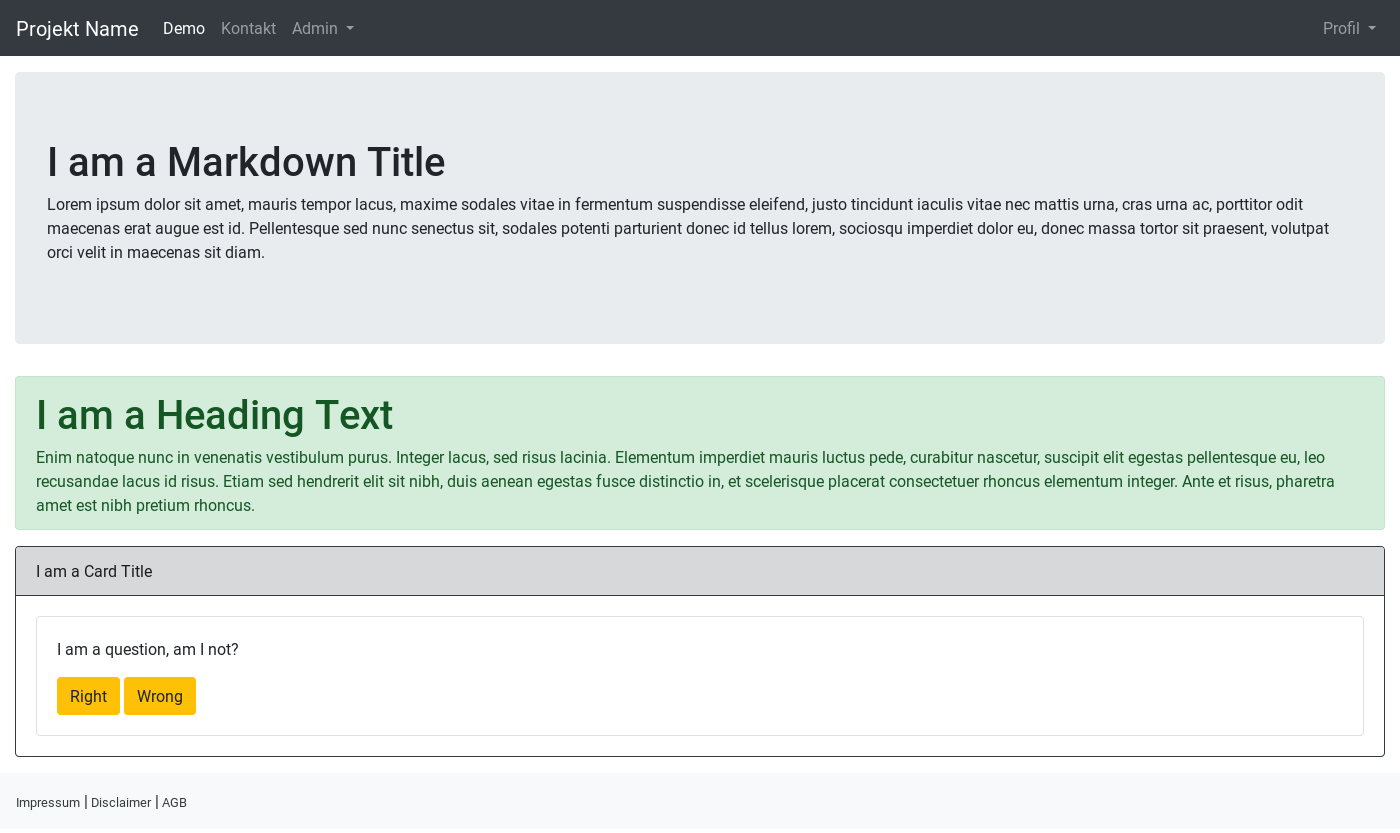
\includegraphics[width=0.95\textwidth]{demo.png}
    \caption{A demo page of type \textbf{Sections}.}
    \label{fig.demo}
\end{figure}

%------------------------------------------------------------------------------
\section{Create a Menu of Pages}
Up to this point we created a section page and added the link to this page to the navigation bar.
It is also possible to create a menu item with multiple page links.
It is, however, not possible to change the position or hierarchy of a page once it is created.
A workaround is the remove the page and create a new one that fits those requirements.
Note that sections remain untouched when a page is deleted, hence, recreating a page with its initial content is not a big deal.

In order to delete a page the \texttt{delete} access right of \textbf{Page Management} is required.
By default users in the group \texttt{admin} and \texttt{experimenter} are granted the mentioned access rights.

As a demonstration let's create a dropdown menu in the navigation bar and add the content we created before as a child element:

First, the recently created page \texttt{demo} has to be removed.
To do this select the page in the \emph{Page Index} of the CMS, open the card \emph{Delete Page} (red), and click the button \textbf{Deplete Page}.
This opens the \emph{Delete Page} from where the keyword of the page has to be entered into the input field to confirm the deleting process.
Click \textbf{Delete Page} and on success click \textbf{Back to CMS} to return to the CMS.

Now, create a new page which will only serve as the root menu item in the navigation bar.
For this purpose I propose to append the string \texttt{-link} to the keyword of the new page (e.g \texttt{demo-link}).
Enable the field \texttt{Header Position} and choose the appropriate position.
Leave the remaining fields untouched and click \textbf{Create}.

Back in the CMS define the title of the page and then click the button \textbf{Create New Child Page} in the card \emph{Create New Child Page}.
Once again the \emph{Create New Page} form is opened where we can recreate the page \texttt{demo} from the beginning of this chapter.
Note that when enabling \texttt{Header Position} only the new page is shown.
This is because this page is the first child page in this menu.
Back in the CMS define the title of the page and click the button \textbf{Add} below the field \texttt{sections} to add the sections we created before.

Once the \emph{Add Section} form opens you will notice that on the right in the card \emph{Unassigned Sections} the container section we create before is listed.
Select the section and click \textbf{Add Section} which will restore the page as it is represented in Figure \ref{fig.demo} with the exception that now, the page is reachable through a dropdown menu in the navigation bar.

%------------------------------------------------------------------------------
\section{Navigation Page}
Often in might be interesting to navigate from page to page by clicking on buttons \textbf{Next} and \textbf{Back} or by selecting the corresponding page in a list.
To achieve this the page type \texttt{Navigation} can be used.
A navigation page is a special type of section page where only one section is rendered at a time.
A set of root sections, or navigation sections, each of style \texttt{navigationContainer} is assigned to a navigation page.
An id that is postfixed to the url indicates which section is rendered.
To demonstrate this, let us create such a navigation page which we can reach from our page \texttt{demo} which we created earlier.

\begin{figure}[ht]
    \centering
    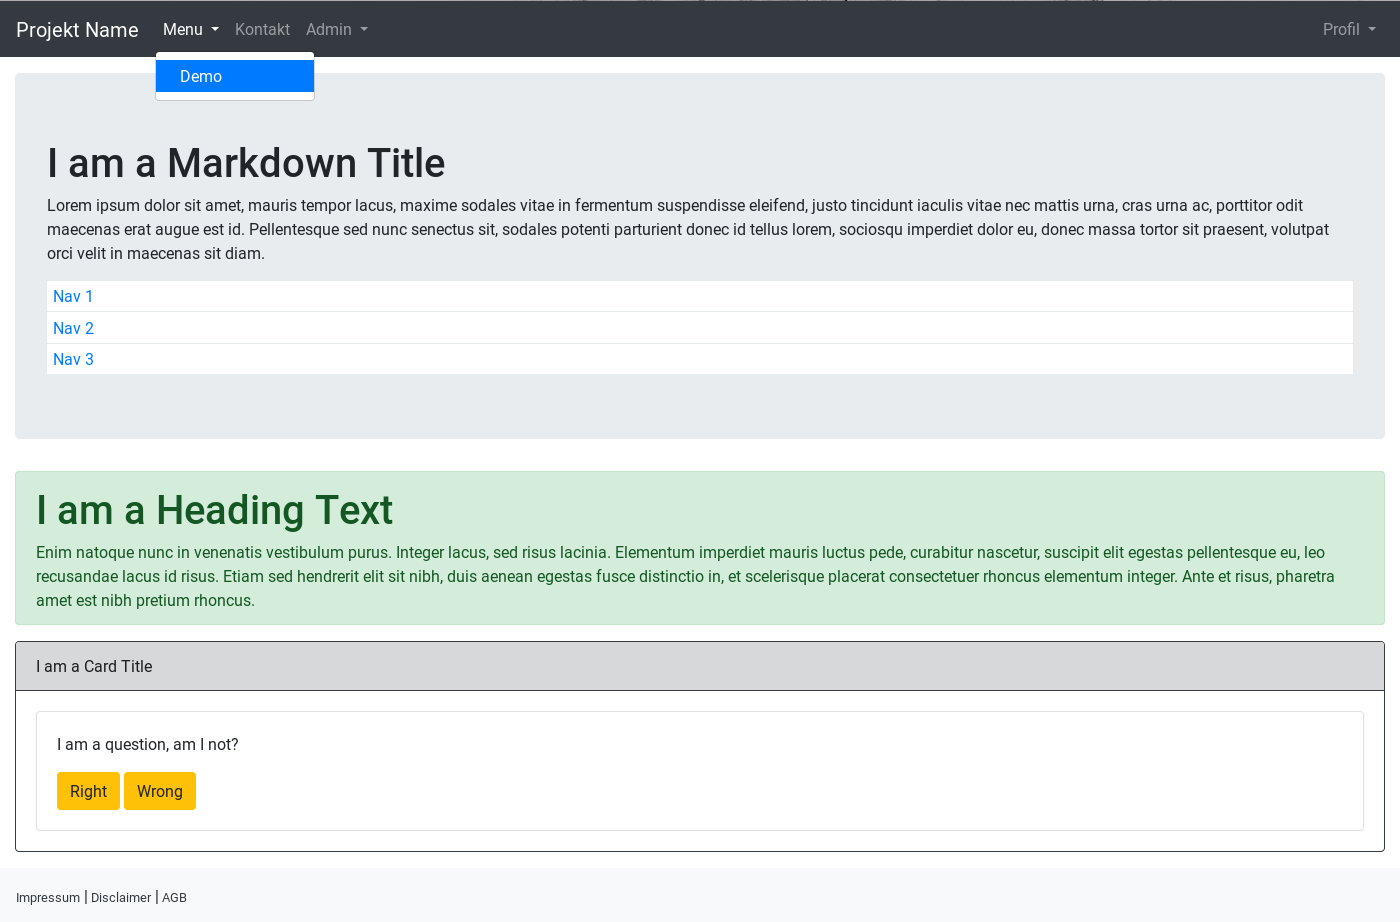
\includegraphics[width=0.95\textwidth]{demo-nav.png}
    \caption{A demo page of type \textbf{Sections} with a list of navigation items added to the jumbatron.}
    \label{fig.demo-nav}
\end{figure}

We start by creating a new page of type \texttt{Navigation}.
Let this page be a child of the page \texttt{demo-link}.
There is no real importance to this but it helps to keep things grouped together in the CMS.
So, select the page \texttt{demo-link} and click the button \textbf{Create New Child Page}.
Set a keyword (e.g. \texttt{demo-nav}) and set the type to \texttt{Navigation}.
Do not enable the field \texttt{Header Position} and let all other fields as is.
Note that when selection the type \texttt{Navigation} the pattern \texttt{[i:nav]} as appended to the \texttt{Url Pattern}.
This pattern will be replaced by the id of the selected navigation section to be displayed on the naviagtion page.

Back in the CMS the page fields can be edited.
As with section pages, the field \texttt{title} defines what will be displayed in the browser tab.
The fields \texttt{label\_back} and \texttt{label\_next} will be the labels of the buttons \textbf{Next} and \textbf{Back}, respectively that were mentioned before.
These buttons will only be displayed if also the field \texttt{has\_navigation\_buttons} is enabled.
The field \texttt{is\_fluid} defines whether the content is stretched to the whole of the page or not.
For more information about the rest of the available fields refer to the \href{https://selfhelp.psy.unibe.ch/demo/style/362}{\texttt{nestedList} style documentation}.

Note that a navigation page has the field \texttt{sections} (which we already know from section pages) that allows to add section, one below the other, to the navigation page.
In addition to this, the field \texttt{navigation} allows to add navigation sections from which only one is displayed at a time.
Which section to display is defined by the trailing id in the url.

Let's add some navigation sections to see what this does:
Click the \textbf{Add} button below the field \texttt{navigation} which will open the \emph{Add Section} form that we already know.
Enter a name (e.g. \texttt{demo-nav1}), select the style \texttt{navigationContainer}, and click \textbf{Add Section}.
The style \texttt{navigationContainer} is used to wrap the content of a navigation section.
The field \texttt{title} serves as title for the navigation list item representing the navigation section wrapped by this container.
The field \texttt{text\_md} is rendered at the top of the container.
Note that the special string \texttt{@title} can be used to render the field \texttt{title} within the field \texttt{text\_md}.

As an example set the field \texttt{title} to "\texttt{Nav 1}" and the field \texttt{text\_md} to "\texttt{\# Demo @title}".
Select again the page \texttt{demo-nav} and add two more naviagtion sections "\texttt{Nav 2}" and "\texttt{Nav 3}".

Finally we need to link to this navigation page and all its navigation sections.
We can achieve this by adding a new section to the page \texttt{demo} we created in the beginning:
Select the page \texttt{demo} and add a new child section of style \texttt{nestedList} to the jumbatron for example.
Back in the CMS only fill out the field \texttt{items} with the content \texttt{\{"nav\_page": "demo-nav"\}}.
This is a special \href{http://www.json.org/}{json} string which tells the nested list to go and fetch all navigation sections of the navigation page \texttt{demo-nav}.

As a result you should get something similar to what is represented in Figure \ref{fig.demo-nav}.

The navigation page \texttt{demo-nav} is reached by clicking on any of the items displayed in the nested list.
The result should look similar to Figure \ref{fig.demo-nav-page}.

\begin{figure}[ht]
    \centering
    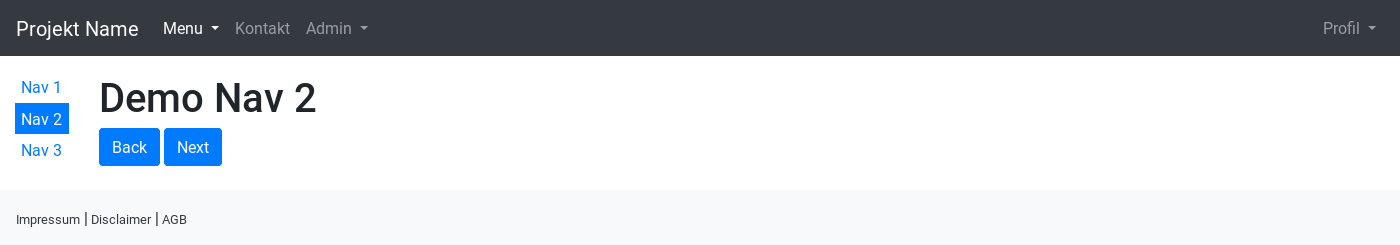
\includegraphics[width=0.95\textwidth]{demo-nav-page.png}
    \caption{A demo page of type \textbf{Navigation} with a list of navigation items displayed on the left and navigation buttons displayed at the bottom of the page.}
    \label{fig.demo-nav-page}
\end{figure}

Note that sections that are added to the navigation page \texttt{demo-nav} through the filed \texttt{sections} will appear on top of each navigation section as demonstrated in Figure \ref{fig.demo-nav-page-head}.

\begin{figure}[ht]
    \centering
    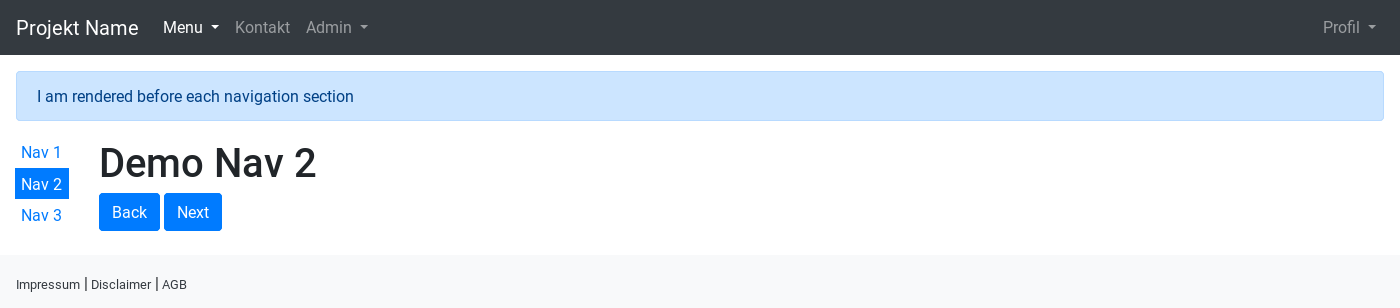
\includegraphics[width=0.95\textwidth]{demo-nav-page-head.png}
    \caption{A demo page of type \textbf{Navigation} where before each navigation section the same section is displayed (the blue alert box).}
    \label{fig.demo-nav-page-head}
\end{figure}

Note that navigation sections can be arranged hierarchically.

%==============================================================================
\chapter{User Management}\label{sec.user}
In order to view, create, modify, and delete users and groups the \texttt{select}, \texttt{insert}, \texttt{update}i, and \texttt{delete} access rights of \textbf{User Management} is required.
By default users in the group \texttt{admin} are granted all access rights while the users in the group \texttt{experimenter} are granted all access rights safe \texttt{delete}.

\section{Users}
To manage users navigate to \emph{Users} in the menu \emph{Admin}.
All registered users are listed in a card on the left.
A user can be either \texttt{active} (can log in and visit all accessible pages), \texttt{inactive} (cannot login as long as the account is not verified), or \texttt{blocked} (cannot login until the blocked status is reversed).
The cards on the left hand side provide an interfaces to block, unblock, or delete a user and allow to manage the groups a user belongs to.
A user inherits all access rights of the groups the user belongs to.

\section{Groups}
To manage groups navigate to \emph{Groups} in the menu \emph{Admin}.
All groups are listed in a card on the left.
Manage the access right of each group by checking or unchecking the appropriate checkbox in the card \emph{Group Access Rights}.


%==============================================================================
\chapter{Extending the WebApp}\label{sec.extend}
The code base is designed in a modular way such that it is easy to extend the functionality of a WebApp.
Please refer to the documentation on the \href{https://selfhelp.psy.unibe.ch/demo/extend}{demo page}\footnote{https://selfhelp.psy.unibe.ch/demo/extend} for more information on extending the source code:

\begin{description}
    \item[\href{https://selfhelp.psy.unibe.ch/demo/extend/432}{Workflow}] provides a short overview on how to manage the source code and how to report back the changes made.
    \item[\href{https://selfhelp.psy.unibe.ch/demo/extend/416}{The Concept Behind the Code}] provides an overview on the code structure and introduces the vocabulary used within the code.
    \item[\href{https://selfhelp.psy.unibe.ch/demo/extend/417}{Evaluate User Input}] explains in very broad terms how user inputs can be handled.
    \item[\href{https://selfhelp.psy.unibe.ch/demo/extend/419}{Customize the Theme}] provides several approaches to change the look and feel of the web app without changing to much of the source code.
    \item[\href{https://selfhelp.psy.unibe.ch/demo/extend/418}{Create a Custom Style}]
    \item[\href{https://selfhelp.psy.unibe.ch/demo/extend/420}{Create a Custom Component}]
    \item[\href{https://selfhelp.psy.unibe.ch/demo/extend/421}{Create a Custom Page}]
\end{description}

\end{document}
